\section{Method}
\label{sec:method}

We introduce a two-stage framework: (i)~deterministic verifiable process reward modelling for teacher RLVR training, and (ii)~reverse-KL reasoning distillation for compact students.
The pipeline remains compatible with a standard SFT $\rightarrow$ GRPO stack~\citep{shao2024deepseekmath}; the optimiser is unchanged, and only reward plugins and distillation objectives are introduced.

\begin{figure*}[t]
    \centering
    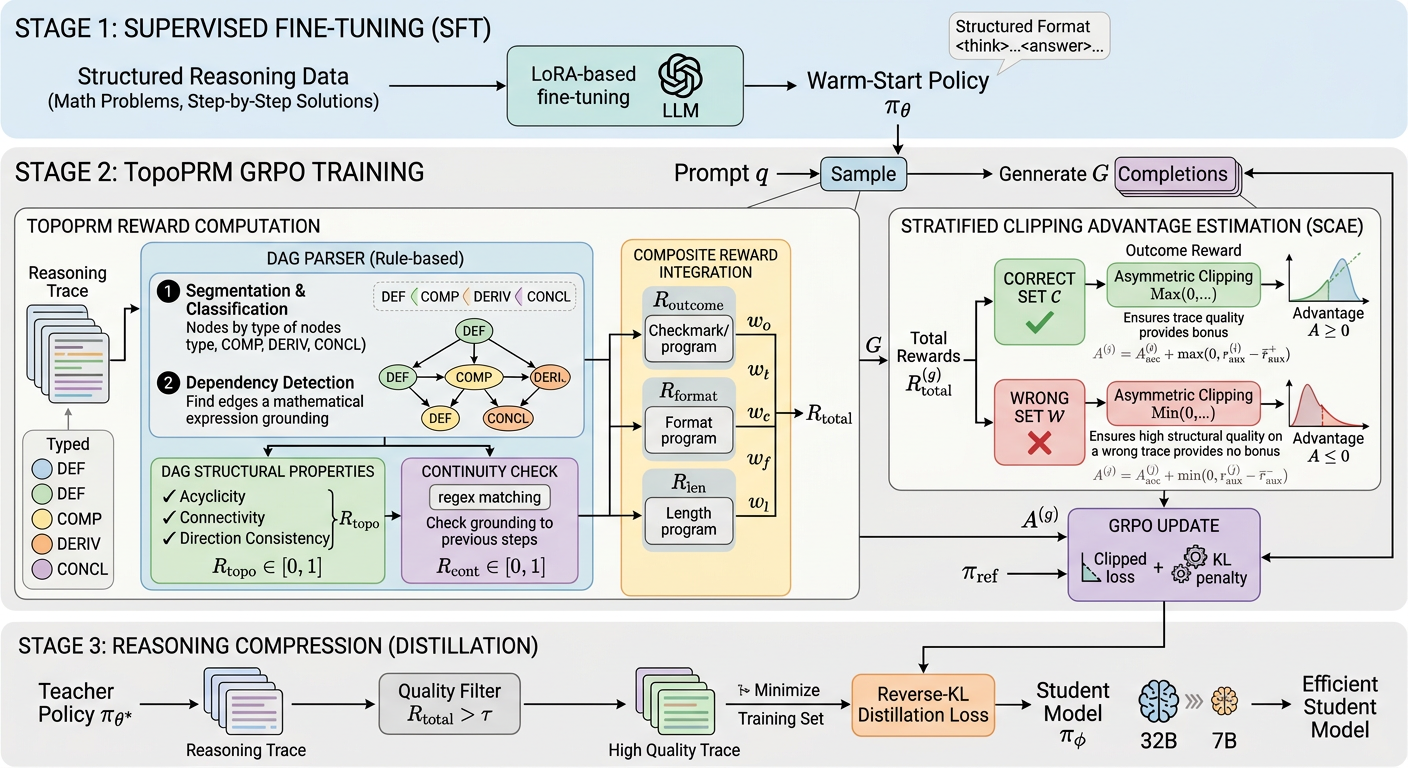
\includegraphics[width=0.98\linewidth]{figures/Ai_Framework.png}
    \caption{Overview of the framework. Stage I trains a teacher with deterministic, verifiable process rewards over extracted dependency DAGs. Stage II applies process-aware filtering and reverse-KL distillation to obtain compact student reasoning.}
    \label{fig:overview}
\end{figure*}

\subsection{Problem Setup}

Given an input $x=(q,s)$, where $q$ is a problem and $s$ is optional context, a policy $\pi_\theta$ generates completion $y$:
\begin{equation}
\label{eq:gen}
y \sim \pi_\theta(\cdot\mid x).
\end{equation}
Outcome-only RLVR uses a sparse correctness signal $r_{\mathrm{out}}(x,y)$, which is effective but often insufficient for controlling reasoning structure. We add deterministic process supervision without introducing learned reward models.

\subsection{Stage I: Verifiable Process Reward Model}

\subsubsection{Deterministic Trace-to-DAG Extraction}

For each reasoning trace $y=(s_1,\ldots,s_T)$ from the \texttt{<think>} block, we apply a deterministic extractor $\mathcal{E}$:
\begin{equation}
\label{eq:extractor}
\mathcal{G}=\mathcal{E}(y)=(\mathcal{V},\mathcal{A}),
\end{equation}
where each node $v_i\in\mathcal{V}$ corresponds to step $s_i$, and each directed edge $(u,v)\in\mathcal{A}$ indicates rule-defined dependency reuse (expression/claim reuse, sequential support, or structural connector).

\textbf{Important scope distinction.} The extracted graph is an inferred dependency DAG induced by deterministic rules; it is not claimed to be a ground-truth proof graph. Thus, deterministic extraction ensures reproducible reward computation, not semantic completeness of dependency recovery.

\subsubsection{Topology Reward (Global Structural Signal)}

We define a topology reward over $\mathcal{G}$:
\begin{equation}
\label{eq:r_topo}
r_{\mathrm{topo}}(\mathcal{G}) =
\lambda_b\,\mathbb{1}[|\mathcal{V}|>0]
+\lambda_a\,\mathbb{1}[\mathcal{G}\ \text{acyclic}]
+\lambda_o\,\mathbb{1}[\rho_{\mathrm{orphan}}(\mathcal{G})=0]
+\lambda_d\,\delta(\mathcal{G})
+\lambda_k\,\kappa(\mathcal{G},\mathcal{G}^{*}).
\end{equation}
Here $\rho_{\mathrm{orphan}}$ measures unsupported conclusion nodes, $\delta$ measures dependency direction consistency, and $\kappa$ is optional reference-edge coverage against a weak reference graph $\mathcal{G}^{*}$ when available.
Default weights in our implementation: $\lambda_b{=}0.20$, $\lambda_a{=}0.15$, $\lambda_o{=}0.15$, $\lambda_d{=}0.15$, $\lambda_k{=}0.25$ (with step-alignment weight $0.10$).
When no reference graph is available, $\lambda_k$ is redistributed proportionally among the remaining terms.

\subsubsection{Continuity Reward (Local Traceability Signal)}

Continuity reward measures local support traceability:
\begin{equation}
\label{eq:r_cont}
r_{\mathrm{cont}}(y)=
\begin{cases}
1.0, & \eta(y)=1,\\
0.8\,\eta(y), & \eta(y)<1,
\end{cases}
\qquad
\eta(y)=\frac{1}{T}\sum_{i=1}^{T}\mathbb{1}[\mathrm{supported}(s_i,s_{<i},q)].
\end{equation}
A step is marked supported if it reuses prior claims/expressions or explicitly cites problem givens under deterministic checks.

\subsubsection{What ``Verifiable'' Means in This Work}

Our use of verifiable reward is operational: once a trace is produced, reward values are computed by deterministic procedures and are therefore reproducible and auditable. This is distinct from semantic proof verification; we do not claim step-correctness guarantees or logical completeness.

\subsection{Stage I Aggregation: Hierarchical Multi-Reward Shaping}

Let
$\mathbf{r}(x,y)=\{r_{\mathrm{out}},r_{\mathrm{topo}},r_{\mathrm{cont}},r_{\mathrm{fmt}},r_{\mathrm{len}}\}$.
A naive weighted sum can mis-rank traces when high process scores compensate for wrong outcomes, and empirically leads to \emph{reward collapse} where batch-level reward variance approaches zero, preventing GRPO from distinguishing good and bad samples.

\paragraph{Hierarchical multiplicative aggregation.}
Instead of linear scalarisation, we adopt a hierarchical formulation that separates base correctness from process-level gain:
\begin{equation}
\label{eq:r_base}
r_{\mathrm{base}} = w_o \cdot r_{\mathrm{out}} + w_f \cdot r_{\mathrm{fmt}} + w_l \cdot r_{\mathrm{len}},
\end{equation}
\begin{equation}
\label{eq:r_total}
r_{\mathrm{total}} = r_{\mathrm{base}} \cdot \bigl(1 + \alpha \cdot \tilde{r}_{\mathrm{topo}} + (1-\alpha) \cdot \tilde{r}_{\mathrm{cont}}\bigr),
\end{equation}
where $\tilde{r}_{\mathrm{topo}}$ and $\tilde{r}_{\mathrm{cont}}$ are batch-level min-max rescaled to $[0,1]$, and $\alpha$ controls the topology--continuity balance (default $\alpha{=}0.6$).
This ensures that process rewards act as a \emph{multiplicative gain} on the base signal rather than an additive offset, preserving answer-correctness primacy while amplifying structural quality differences.

\paragraph{Anti-collapse mechanisms.}
To prevent reward collapse during GRPO training, we employ three complementary mechanisms:
(i)~batch-level min-max rescaling ensures process reward components have sufficient spread;
(ii)~reward temperature scaling ($\tau{=}2.0$) amplifies small differences: $r \leftarrow \mu + (r - \mu) \cdot \tau$;
(iii)~a minimum-variance guard injects small Gaussian noise ($\epsilon{=}0.01$) when batch reward standard deviation falls below a threshold ($\sigma_{\min}{=}0.005$).

\paragraph{Optional: GAT-based topology scoring.}
As an alternative to rule-based topology reward computation, we provide a lightweight Graph Attention Network (GAT) scorer.
Given the extracted DAG, each node receives features comprising Laplacian eigenvector position encoding (top-$k{=}8$), normalised degree, topological depth, and step-level text features.
A two-layer GAT with 4 attention heads and hidden dimension 64 produces a graph-level quality score via mean readout.
The GAT scorer operates independently of LLM training and can be used in pure or hybrid mode (averaging with rule-based scores).

\paragraph{Correctness-first stratification (SCAE-style implementation).}
\begin{equation}
\label{eq:scae_partition}
\mathcal{C}=\{i\mid r_{\mathrm{out}}^{(i)}\ge\tau\},
\qquad
\mathcal{W}=\{i\mid r_{\mathrm{out}}^{(i)}<\tau\}.
\end{equation}
Within each stratum, we standardize and asymmetrically clip:
\begin{equation}
\label{eq:scae_shape}
\tilde{r}^{(i)}=
\begin{cases}
\mathrm{clip}(z^{(i)},0,1.5), & i\in\mathcal{C},\\
\mathrm{clip}(z^{(i)},-1.5,0), & i\in\mathcal{W}.
\end{cases}
\end{equation}
This guarantees that answer-correct traces remain non-negative and answer-incorrect traces remain non-positive after shaping.

\subsection{Stage II: Reverse-KL Reasoning Distillation}
\label{sec:compression}

Let $\pi_T$ be the teacher after Stage~I and $\pi_S$ the student.
We first build a filtered set $\mathcal{D}_f$ by retaining teacher traces that satisfy process-aware quality thresholds (composite reward $R_{\mathrm{total}} > 0.7$).
Distillation minimises reverse KL:
\begin{equation}
\label{eq:distill}
\mathcal{L}_{\mathrm{RKL}}=
\mathbb{E}_{x\sim\mathcal{D}}\left[
D_{\mathrm{KL}}\!\left(\pi_S(\cdot\mid x)\,\|\,\pi_T(\cdot\mid x)\right)
\right].
\end{equation}
Reverse KL is mode-seeking: it encourages $\pi_S$ to concentrate on high-probability teacher modes rather than averaging over diverse outputs~\citep{sang2026opsdc}.
In our setting, this compresses graph-enriched teacher reasoning behaviour into compact chain-like student reasoning without requiring explicit DAG output from the student.

\begin{algorithm}[t]
\caption{Training Pipeline}
\label{alg:topoprm}
\begin{algorithmic}[1]
\Require Base model $\pi_0$, SFT set $\mathcal{D}_{\mathrm{sft}}$, RL prompts $\mathcal{D}_{\mathrm{rl}}$
\Ensure Teacher $\pi_T$ and optional student $\pi_S$
\State Train $\pi_\theta \leftarrow \mathrm{SFT}(\pi_0,\mathcal{D}_{\mathrm{sft}})$
\For{each GRPO batch on $\mathcal{D}_{\mathrm{rl}}$}
  \State Sample completions and extract dependency DAGs by deterministic parser
  \State Compute $r_{\mathrm{out}},r_{\mathrm{topo}},r_{\mathrm{cont}},r_{\mathrm{fmt}},r_{\mathrm{len}}$
  \State Aggregate via Eq.~\ref{eq:r_total} and shape via Eq.~\ref{eq:scae_shape}
  \State Update policy using stock GRPO with shaped rewards
\EndFor
\State Set teacher $\pi_T \leftarrow \pi_\theta$
\If{distillation enabled}
  \State Filter teacher traces by process-aware criteria to build $\mathcal{D}_f$
  \State Train student $\pi_S$ by minimizing Eq.~\ref{eq:distill}
\EndIf
\end{algorithmic}
\end{algorithm}
